\documentclass[tikz,border=3mm]{standalone}
\usepackage[T1]{fontenc}
\usetikzlibrary{positioning,shapes.geometric}
\begin{document}
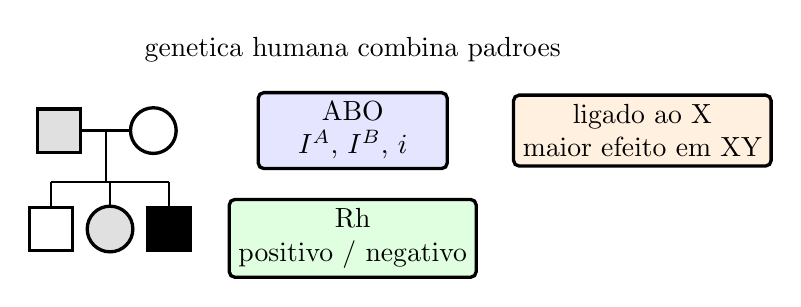
\begin{tikzpicture}[node distance=0.7cm]
  \tikzstyle{male}=[draw,very thick,minimum size=0.55cm]
  \tikzstyle{female}=[draw,very thick,circle,minimum size=0.58cm]
  \tikzstyle{box}=[draw,rounded corners=2pt,very thick,align=center,minimum width=2.4cm,minimum height=0.7cm]
  \node[male,fill=black!12] (m1) at (0,0) {};
  \node[female] (f1) at (1.2,0) {};
  \draw[thick] (m1) -- (f1);
  \draw[thick] (0.6,0) -- (0.6,-0.65);
  \node[male] (s1) at (-0.1,-1.25) {};
  \node[female,fill=black!12] (d1) at (0.65,-1.25) {};
  \node[male,fill=black] (s2) at (1.4,-1.25) {};
  \draw[thick] (-0.1,-0.65) -- (1.4,-0.65);
  \draw[thick] (-0.1,-0.65) -- (s1);
  \draw[thick] (0.65,-0.65) -- (d1);
  \draw[thick] (1.4,-0.65) -- (s2);
  \node[box,fill=blue!10,right=1.0cm of f1] (abo) {ABO\\$I^A$, $I^B$, $i$};
  \node[box,fill=green!12,below=0.35cm of abo] (rh) {Rh\\positivo / negativo};
  \node[box,fill=orange!12,right=0.8cm of abo] (x) {ligado ao X\\maior efeito em XY};
  \node[align=center,above=0.25cm of abo] {genetica humana combina padroes};
\end{tikzpicture}
\end{document}
